\documentclass[a4paper,12pt,oneside]{report}

\usepackage{fancyhdr}
\usepackage[magyar]{babel}
\usepackage{t1enc}
\usepackage[utf8]{inputenc}
\usepackage{graphicx}
\usepackage{todonotes}
\usepackage[section,numbib]{tocbibind}
\usepackage{formai_kovetelmenyek}

\title{\textbf{Ülésszervezést és jegyzőkönyv-írást támogató keretrendszer készítése}}
\author{Fási Gábor\\\\Témavezető: Dulai Tibor}
\date{}

%fattyú- és árvasorok büntetése, ha nagyobb, akkor jobban próbálja elkerülni
\widowpenalty=300
\clubpenalty=300

\graphicspath{{./kepek/}}

\begin{document}
\setcounter{chapter}{1}

\maketitle

\listoftodos

\tableofcontents
\thispagestyle{empty}
\pagebreak

\setcounter{page}{1} %innentől indul az oldalszámozás
\section{A feladat felvázolása}

Témám egy olyan rendszer elkészítése, mely böngészőn keresztül használható, a megfelelő jogosultságú felhasználók képesek ülést hirdetni helyszínnel, időponttal, majd erre résztvevőket meghívni, akik erről automatikus értesítést kapnak. Szintén a rendszer feladata a lefolyt ülések jegyzőkönyvei elkészítésének segítése, ezek megőrzése és megfelelő feltételek esetén nyilvánossá tétele.

A rendszer fő haszonélvezője a Pannon Egyetem Hallgatói Önkormányzata lesz, de célom a lehetőség általánosítás, hogy a későbbiekben bárki könnyen és gyorsan az egyedi igényeihez tudja szabni és használatba venni.

\section{Hasonló rendszerek}

Számos jegyzőkönyvvezető rendszer érhető el már magyar nyelven is, de ezek többsége másfélére specializálódott, mint az én rendszerem; például mérési-, verseny vagy vizsgajegyzőkönyv-készítésre.

Három darab ülésjegyzőkönyv-készítő funkcionalitással bíró rendszert találtam, melyek magyar készítésűek:

\begin{itemize}

    \item \emph{AC-TMTR, avagy az Albacomp Testületi Munkát Támogató Rendszer}\cite{website:actmtr}\\
    Önkormányzatok számára készült, honlapjuk szerint ,,Az AC-TMTR a teljes demokratikus döntéshozatali folyamat támogatására alkalmas az előterjesztések kezelésétől a döntések végrehajtásáig''.\\
    A rendszer tudása messze több, mint jegyzőkönyvkészítés, Lotus Notes alapon működik.
    
    \item \emph{InterMap e-FORTE}\cite{website:eforte}\\
    Fő célcsoportja a polgármesteri hivatalok, felső államigazgatás és nagyvállalatok vezetése, ennek tudása is jelentősen meghaladja a jegyzőkönyvkészítést és ülésszervezést.\\
    Webalapú, ASP.NET nyelven készült.
    
    \item \emph{eKÖZIG döntéstámogató rendszer}\cite{website:ekozig}\\
    Szintén a közigazgatás a fő célcsoport, nagyméretű és bonyolult rendszert eredményezve.\\
    Webalapú, ASP nyelven íródott.
    
\end{itemize}

A fenti rendszerek mindegyike fizetős, valamint a mögöttes technológia is \textendash{} az operációs rendszer (Windows) és a futtatókörnyezet (ASP, ASP.NET) egyaránt komoly beruházást igényel a bevezetéskor.

\section{Rendszerterv}

A rendszer három fő modulra bontható:

\begin{enumerate}
    \item Felhasználókezelés, authentikáció és authorizáció
    \item Ülések hirdetése, kezelése
    \item Jegyzőkönyvírás
\end{enumerate}

\subsection{Felhasználókezelés, authentikáció és authorizáció}

Az alkalmazás zárt, azaz nincs szabad regisztráció, csak az adminisztrátorok hozhatnak létre új felhasználót, illetve ők tudják a létezőket módosítani. A rendszer a kényelmes, gyors és biztonságos bejelentkezésre a Google OpenID rendszerét használja, így nem kell például jelszavak biztonságos tárolásáról gondoskodnunk. Minden HÖK tag rendelkezik egy Google Apps fiókkal.

Ennek a modulnak a feladata az OpenID bejelentkezési folyamat megvalósítása, a kapott adatok alapján a felhasználóhoz párosított jogosultsági szint ellenőrzése a rendszer használata során. Szintén ide tartozik a felhasználók adminisztrátorok általi kezelése.

\subsection{Ülések hirdetése, kezelése}

Az ülések rendelkeznek fix számú adattal, mint a rövid leírásuk, időpontjuk és a helyszínük. Megfelelő jogosultsággal rendelkező felhasználók képesek a fenti adatok megadása után ülést hirdetni, meghívottakat megadni. Opcionális adat még az ülés hosszú leírása, itt lehet például megadni a tervezett napirendi pontokat; valamint lehetőség van dokumentumok feltöltésére, ha valami anyagot előzetesen tanulmányozni kell a résztvevőknek.

A rendszer a hirdetett üléseknek létrehoz egy bejegyzést a Google Naptár alkalmazásában, melyre meghívja a résztvevőket, így az bekerül az ő naptárukba is, valamint erről értesítő levelet kapnak.

\subsection{Jegyzőkönyvírás}

A lezajlott ülésekhez készíthető jegyzőkönyv, de természetesen ülés nélkül is lehet jegyzőkönyvet létrehozni (korábbi ülések, vagy ha a szervezés valamely oknál fogva a rendszeren kívül történt).

A jegyzőkönyvek rendelkeznek ugyanazokkal az alapadatokkal, mint az ülések, valamint tetszőleges számú bejegyzéssel, melyekből három típust különböztetünk meg: napirendi pont, felszólalás valamint szavazás. Mind más adatokkal rendelkezik, a rendszernek kezelnie kell ezt, valamint a bejegyzések egymás közti sorrendjét.

A papír alapú iktatást elősegítendő lehetőség van az elkészült jegyzőkönyvek pdf formátumú exportálására.

Szintén e modul feladata a nyilvános ülések kész jegyzőkönyveinek publikálása, bárki számára elérhetővé tétele.

\section{Választott technológia}

Feladatom tervezése során hangsúlyt fektettem arra, hogy nyílt forráskódú, ingyenes rendszerekre építsem a megoldásom. A hardverköltségtől eltekintve, amely mindenképpen jelen van, az ilyen szerverek összeállítása a lehető legolcsóbb, illetve szakemberek is bőven állnak rendelkezésre. Így esett választásom a PHP nyelvre és a Symfony2 keretrendszerre.

A választott követelményeimnek megfelelő webszerverekből az egyetem már most is rendelkezik több darabbal, és persze hozzájuk értő rendszergazdákkal is, így a rendszer majdani bevezetésének a költsége minimális.

\subsection{PHP}

A php ma az egyik legelterjedtebb programozási nyelv, melyet weboldalak készítésére használnak. Rengeteg kezdőknek szóló leírás van róla, minden webfejlesztő ismeri legalább az alapjait. Bőségesen áll rendelkezésre akár ingyenes tárhely is, ahová felrakhatjuk az elkészült programunkat.

A 2008-ban megjelent 5.3-as verzióval a nyelvbe bekerült a névterek támogatása, valamint a garbage collector algoritmusa is sokat javult, jelentős teljesítmény\-növe\-kedést eredményezve. A feladatom minimum követelménye az 5.3.7-es verzió, ebben javítottak egy, a bcrypt modulban levő hibát, mely hibás (viszonylag könnyen törhető) jelszókódolást eredményezett.

\subsection{Symfony2}

A Symfony az egyik nagy keretrendszer a php világában. Első verziója 2005-ben jelent meg, csak ragasztó volt egy maréknyi könyvtár közt, azok együttes használatát segítendő. Folyamatosan fejlődött, olyan nagy oldalak hasz\-nálták, mint a Yahoo!\cite{website:symfony_yahoo} és a Dailymotion\cite{website:symfony_dailymotion}. Az 1.4-es ága 2009-ben jelent meg, és egészen 2012 novemberéig rendelkezett támogatással.

A Symfony2 hosszas fejlesztést követően jelent meg 2011 júliusában. Az egyik első nagy keretrendszer volt, mely a php5.3 új lehetőségeit kihasználva lett az alapoktól újraírva. Fejlődése a közösség bevonásával történt, több, mint 250 önkéntes segített be. Mostanra 600 feletti a fejlesztésben részt vevők száma.

A rendszerem fejlesztése a 2.1-es verzióban történt. A készítés utolsó hónapjaiban adták ki a 2.2-es verziót számos visszafelé nem kompatibilis változtatással, ezért nem frissítettem rá \textendash{} a 2.1-es változat 2013 közepéig élvez hivatalos támogatást, így a rendszer további fejlesztése során mindenképpen megfontolandó a 2.2-re átállás.

A Symfony remekül együtt tud működni a Doctrine\cite{website:doctrine} ORM-el, ezzel lehetővé téve, hogy az alkalmazásunk számára észrevétlenül lecseréljük az adatbázis-szerverünk valamely más típusúra. A tábláink szerkezetét egy egységes módon kell megadnunk, és az illesztőfüggő kódot a Doctrine legenerálja nekünk.

\subsection{Bootstrap}

A Twitter által megalkotott Bootstrap\cite{website:bootstrap} css keretrendszer segítségével könnyen és gyorsan hozhatunk létre egységes, jól kinéző webalkalmazásokat. Beépítve tartalmaz egyszerű, de jól használható stílusokat a webfejlesztés szinte minden területére, az alapkinézet megalkotásától az űrlapmezők formázásáig. Élénk közösség alakult ki körülötte, így a korábban nem lefedett területekre is számos megoldás létezik mostanra. A kezdetek óta kiegészült egy maréknyi javascript könyvtárral is, melyekkel egyszerűen tudunk például dialógusablakokat vagy hasonló, gyakori feladatokat megoldani.

\section{Kritikus részek}

A következőkben megemlítem a rendszer kritikus pontjait, illetve hogy milyen tervvel rendelkezem ezek megoldására.

\subsection{OpenID authentikáció}

Az OpenID\cite{website:openid_specifikacio} egy viszonylag összetett protokoll sok hibázási lehetőséggel. Szerencsére több készen elérhető megoldás is létezik, ezek közül nem egy pedig minimális konfiguráció után kész együttműködni a Symfony2 biztonsági komponensével köszönhetően annak, hogy készítettek hozzá kiterjesztést (a Symfony terminológiában Bundle-t). Ezek közül az FpOpenIdBundle\cite{website:fpopenidbundle}-t választottam.

\subsection{Jogosultságkezelés}

A jogosultságok kiosztásában olyan rugalmasnak kell lennünk, amit egy egyszerű, felhasználókat csoportokra bontó megoldás nem tesz lehetővé. Az egyeztetések során hamar kiderült, hogy több olyan felhasználó is lesz, aki az eredeti rendszer szerint nem hirdethetne ülést (mert nem kari elnök), de ezt mégis lehetővé kell tenni számára.

A Symfony2 Security komponense nagyon finom jogosultság-szabályoztást tesz lehetővé onnantól, hogy egy oldalt valaki csak megfelelő joggal ér el, odáig, hogy egy adott adatbázis-rekord valamely mezőjéhez hozzáférhet-e.

\subsection{Google Naptár együttműködés}

Az API, amivel eseményeket lehet létrehozni és arra meghívottakat hozzáadni\cite{website:gcal_event_api} nincs túlbonyolítva, és a Google ad php-hoz hivatalos klienskönyvtárat\cite{website:google_api_client}. Ennek segítségével fogok létrehozni egy Symfony2 szolgáltatást, mellyel a rendszer bármely részéről könnyen tudok majd a Naptárral kapcsolatba lépni.

\subsection{PDF exportálás}

Webes rendszerek esetén gyakran előforduló kérés, hogy valamely generált dokumentumot lehessen pdf-ben is letölteni; így nem meglepő, hogy számos Symfony2 Bundle foglalkozik ezzel a feladattal.

A választásomtól függően vagy egy könyvtár megfelelő függvényeit hívva, úgymond kézzel állítom össze a kimenetet, vagy html-ből tudom a pdf-et generáltatni. A végleges választás további kísérleteket igényel.

\section{Felületterv}

Az következőkben bemutatom a rendszer három várhatóan leggyakrabban látogatott képernyőjét. Az elrendezése mindegyiknek ugyanaz: felül egy menüsáv, ahol a bejelentkezett felhasználó jogosultsági szintjétől függően látszanak a menüpontok.

\subsection{Kezdőlap}

Bejelentkezés után minden felhasználó erre az oldalra érkezik. Áttekintő táblázatot kap az elkövetkező üléseiről, illetve azon jegyzőkönyveiről, melyek már létre lettek hozva, de még nincsenek lezárva.

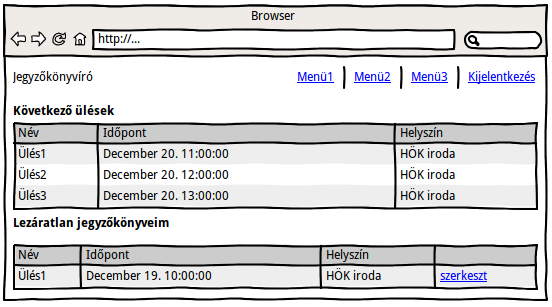
\includegraphics[width=\textwidth]{wireframe-kezdolap}

\subsection{Üléshirdetés}

Ezen a képernyőn lehet megadni az ülés alapadatait és résztvevőket meghívni.

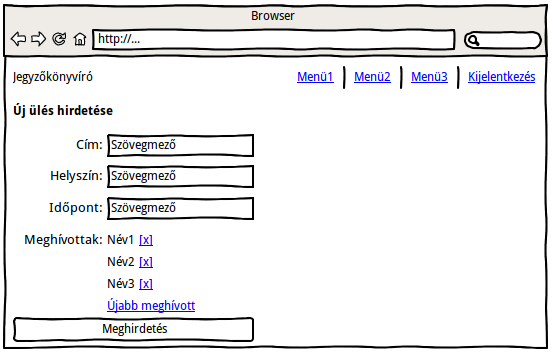
\includegraphics[width=\textwidth]{wireframe-uleshirdetes}

\subsection{Jegyzőkönyvírás}

Itt tudja az írással megbízott felhasználó felvinni a jegyzőkönyv elemeit, melyek sorrendfüggően egymás alatt látszanak.

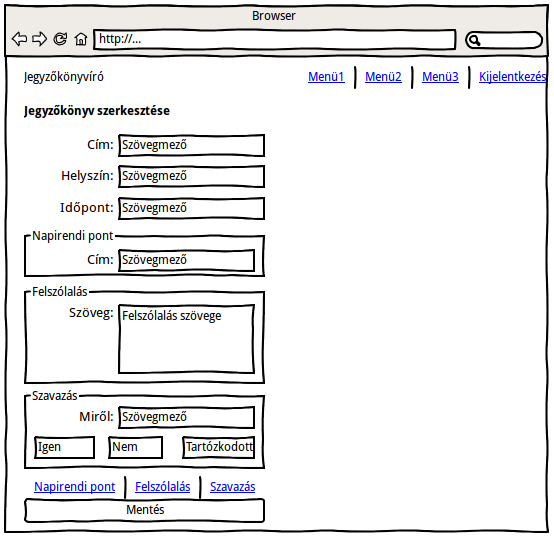
\includegraphics[width=\textwidth]{wireframe-jegyzokonyvszerkesztes}

\section{Jogosultságok leírása}

Néhány mondatban szót ejtek a rendszer által kezelt jogosultságokról, illetve hogy kik lesznek a jellemző tulajdonosai.

%csillagozva nem kap számozást, és a tartalomjegyzékbe sem kerül be
\subsection*{Felhasználó}

Az alapszintű jogosultság, hozzáfér a rendszerhez, tud jegyzőkönyveket létrehozni és megírni, illetve azon ülések részleteihez és feltöltött anyagaihoz hozzáférni, ahol meghívottként szerepel.

Nem kell külön kiosztani, megkapja mindenki, aki a rendszerhez hozzáféréssel rendelkezik.

\subsection*{Üléshirdető}

A fentieken kívül tud még ülést hirdetni, annak jegyzőkönyvírásával megbízni valakit, illetve természetesen az üléseinek adatait szerkeszteni, azokhoz dokumentumokat feltölteni.

Jellemzően a kari HÖK elnökök kapják majd ezt a jogot, de rajtuk kívül más személyek is, akik valamely vezető tisztségben vannak.

\subsection*{Adminisztrátor}

A fentieken kívül képes a felhasználók kezelésére, adja meg adataikat (teljes név, HÖK-ön belüli tisztség), illetve osztja ki a jogosultságaikat. Képes tetszőleges ülés adatait és meghívottait módosítani.

Kezdetben egyetlen ilyen jogú felhasználó lesz, a későbbiekben ez az egy igény szerint tud létrehozni újabbakat.

\section{Jegyzőkönyv létrehozásának folyamata}

Egy jegyzőkönyv létrehozása az ülés hirdetésétől kezdve a következő lépésekből áll:

\begin{enumerate}
  \item \emph{Ülés hirdetése}\\
    Egy arra jogosult személy meghirdet egy ülést, megadja annak alapadatait (név, helyszín, napirendi pontok), meghívja a résztvevőket.
    
  \item \emph{Ülés jegyzőkönyvírójának megadása}\\
    Az ülés hirdetője a meghívottak közül kiválasztja a jegyzőkönyvírással megbízott személyt, valamint a jegyzőkönyv két hitelesítőjét.
    
  \item \emph{Jegyzőkönyv alapadatainak megadása}\\
    A jegyzőkönyv írója létrehozza az új jegyzőkönyvet és megadja annak alapadatait. Alternatívaként kiválaszthatja, hogy melyik ülés jegyzőkönyvét írja, ekkor a rendszer az ismert adatokat átemeli onnan.

  \item \emph{Jegyzőköny megírása}\\
    A megbízott megírja a jegyzőkönyvet tetszőleges számú bejegyzést hozva létre.
    
  \item \emph{Jegyzőkönyv lezárása}\\
    A jegyzőkönyv írója a folyamat végén lezárja a jegyzőkönyvet, innentől ez nem módosítható. Nyilvános ülés esetén a kész jegyzőkönyv publikálásra kerül, illetve e-mailben az elkészültéről értesítést kap az Ellenőrző Bizottság.
  
\end{enumerate}

A folyamat úgy van kitalálva, hogy két felhasználóra oszlanak a feladatok: az ülés hirdetőjére és a jegyzőkönyv írójára. Természetesen a két személy lehet ugyanaz, ha az ülés hirdetője a jegyzőkönyvíró szerepét önmagának osztja ki.

\section{Tesztelési terv}

A Symfony2 remekül támogatatja az egység- és funkcionális tesztek írását. Ezt lehetőségeimhez mérten igyekszem kihasználni megelőzve azt, hogy a fejlesztés későbbi részeiben valami már működő funkcionalitást elrontsak.

\todo[inline]{Tesztelésről részletesebben}
Szintén hasznát fogom venni a Travis-CI szolgáltatásnak, melynek lényege az, hogy minden verziókövetőbe történő commit után automatikusan lefuttatja a teszteket akár több PHP verzión, illetve adatbázis-szerveren.

Emellett amint a rendszer eléri a megfelelő fejlettségi szintet, telepítésre kerül egy alkalmas szerverre, hogy valós felhasználók is elkezdhessék annak próbálgatását és visszajelzések küldését.

\section{Fejlesztési terv}

A rendszer moduljainak tervezett fejlesztési sorrendje az egymásraépülések miatt a következő:

\begin{enumerate}
  \item \emph{Felhasználók}\\
    Ebben a szakaszban készül el a bejelentkezési folyamat, a felhasználóhoz jogainak hozzárendelése, valamint a felhasználók kezelésére szolgáló rész: azok listázása, új felvétele, létezők szerkesztése.
    
  \item \emph{Ülések}\\
    Elkészül az üléshirdetési folyamat meghívással, egyelőre a Google Calendar integráció nélkül. Működik a dokumentumfeltöltés, valamint az ülések listázása több szempontból, mint például a saját üléseim, vagy azok, amelyekre meghívtak.
    
  \item \emph{Jegyzőkönyvek}\\
    Megvalósításra kerül a jegyzőkönyvek készítésére szolgáló modul. Lehet újat létrehozni csak úgy, illetve üléshez kapcsolva is. A pdf exportálás későbbre marad.\\
    Előzetes becsléseim szerint ez a szakasz lesz a legidőigényesebb.
    
  \item \emph{Tesztelés}\\
    A rendszer alapvető funkciói elkészültek, így az telepíthető egy arra alkalmas HÖK-ös szerverre, hogy elkezdődhessen az éles üzemre való felkészítés, illetve hogy valós felhasználói vélemények alapján tudjam a működést finomhangolni.
    
  \item \emph{Naptáresemény és exportálás}\\
    Megvalósul a Google Naptárral kommunikáló szolgáltatás, hogy a hirdetett ülésekről ott is létrejöjjön esemény, valamint a kész jegyzőkönyvek PDF formátumban történő exportálási lehetősége.
\end{enumerate}

\renewcommand{\bibname}{Irodalomjegyzék}
\bibliographystyle{plain}
\bibliography{irodalomjegyzek}

\end{document}
